\chapter{Privacyrisico's bij klassieke aanbevelingsystemen}
\label{privacyklassiek}

\section{Klassieke aanbevelingssystemen}
\label{sec:klassiek}
In wat volgt beschrijven we de verschillende soorten klassieke aanbevelingssystemen, en geven voor elke soort een korte uitleg waarin de werking ervan aan bod komt. Voor meer informatie omtrent de precieze werking wordt doorverwezen naar de vakliteratuur. \\
\\
Er wordt onderscheid gemaakt tussen de volgende types:
\subsection{Niet-gepersonaliseerde statistieken}
Dit is de meest eenvoudige vorm van een aanbevelingssysteem. Statistieken van ratings van de community zoals het gemiddelde aantal sterren van een beoordeling of items met het grootste aantal "vind-ik-leuk"'s zijn alomtegenwoordig. Andere statistieken die populair zijn, zijn productassociaties in de vorm van “mensen die x leuk vonden, vonden ook y leuk”. Externe community data, zoals bijvoorbeeld meest verkochte items, wordt ook gebruikt. Hoewel de niet-gepersonaliseerde statistieken duidelijk hun beperkingen hebben, zijn ze effici\"ent en kunnen ze erg nuttig zijn. 
\subsection{Content-based recommenders}
Het basisidee van inhoud-gebaseerde aanbevelingssystemen is om items te modelleren als vectoren in een meerdimensionale ruimte. Deze ruimte heeft als dimensies de relevante attributen van de items. De voorkeuren van de gebruiker wordt vervolgens voorgesteld als een vector in deze ruimte, de zgn.~\textit{uservector}. De ligging van de uservector wordt aan de hand van de ratings die de gebruiker heeft gegeven aan items met bepaalde attributen. De interessante items worden meestal gevonden door die items te nemen waarvan de hoek tussen de itemvector en de uservector klein is. 
\subsection{Kennis-gebaseerde recommenders}
De gebruiker die aanbevelingen vraagt zal zijn voorkeuren aan het systeem geven. De gebruiker kan op de aangeboden items feedback geven zodat het systeem zijn aanbevelingen kan aanpassen.
\subsection{Collaborative Filtering recommenders}
\subsubsection{User-User Collaborative recommenders}
Bij user-user collaborative recommenders wordt de smaak van gebruikers vergeleken op basis van hun gegeven ratings met een  correlatieco\"effici\"ent zoals deze van Pearson \cite{?}. Als een gebruiker aanbevelingen vraagt, worden de gebruikers met een gelijkaardige smaak bepaald. De score voor een item wordt berekend door het gewogen gemiddelde te nemen van de scores voor dat item van de gebruikers met gelijkaardige smaak.
\subsubsection{Item-Item Collaborative recommenders}
Om een score voor een item te vinden voor een gebruiker wordt eerst gekeken naar de items waar deze gebruiker reeds een rating voor heeft. Indien het gezochte item volgens andere gebruikers gelijkaardig is aan reeds beoordeelde items (i.e.~een gelijkaardige score heeft voor hen), neemt men het gewogen gemiddelde van de ratings van deze items.
\subsection{Andere aanbevelingssystemen}
\subsubsection{Demografic recommenders}
Als een persoonlijke voorkeur niet gekend is wordt afgegaan op kenmerken als leeftijd, geslacht en land van herkomst om aanbevelingen te genereren op basis van een stereotype.
\subsubsection{Social recommenders}
Deze aanbevelingssystemen maken gebruik van de vriendschapsbanden van een sociaal netwerk omdat aangenomen wordt dat vrienden gelijkaardige interesses hebben.
\subsubsection{Hybrid recommenders}
Zoals de naam aangeeft worden hier verschillende aanbevelingssystemen gecombineerd. Doel is om betere aanbevelingen te produceren en de nadelen van de onderliggende systemen weg te werken.

\subsection{Singular Value Decomposition}
Singular Value Decomposition of singulierewaardenontbinding is een wiskundige techniek die toelaat een $m \times n$ matrix $A$ op te splitsen in een product van drie matrices. Respectievelijk: een $m \times m$ \emph{user-feature} matrix $U$, een $m \times r$ matrix $\Sigma$ met de singuliere waarden op de diagonaal en een $r \times r$ \emph{item-feature} matrix $V$.\\ 
Deze techniek kan uitgevoerd worden op een traditionele user rating matrix om de smaken van de gebruikers niet vast te leggen als scores op bepaalde trefwoorden maar eerder in een aantal dimensies die verschillende trefwoorden overstijgen. De singuliere waarden op de diagonaal van $\Sigma$ geven de belangrijkheid van deze bepaalde dimensie aan. Een deel van deze waarden is dicht bij 0 en dus kunnen deze  dimensies verwaarloosd worden en de matrix verkleind worden naar $k$ rijen en kolommen. De scores in de $U$ en de $V$ matrices op deze verwaarloosde dimensies kunnen ook weggelaten worden. Dit zorgt voor minder computationeel werk en een compactere datarepresentatie. 
\section{Evaluatie van aanbevelingssystemen}
Een veelgebruikte basismetriek is de Mean Absolute Error (MAE) of de gemiddelde absolute fout. Een bestaande rating voor een item wordt tijdelijk ``onzichtbaar'' gemaakt voor het systeem, waarna het systeem aangeeft welke score het aan dat item zou geven op basis van alle andere bekende ratings. Het verschil tussen de oorspronkelijke (tijdelijk weggelaten) rating en de nieuw berekende score is dus de fout. We berekenen het gemiddelde van de fouten voor elke rating en zo bekomen we het MAE. Een vergelijkbaar alternatief is de Mean Squared Error (MSE), die door kwadratering de grote fouten meer afstraft. De Root Mean Squared Error (RMSE) is hiervan de vierkantswortel zodat er een waarde bekomen wordt in de meer intu\"itieve originele schaal.
\begin{equation}
\text{MAE} = \frac{\sum_{\text{ratings}} (\text{prediction} - \text{rating})}{\#\text{ratings}}
\end{equation}
\begin{equation}
\text{MSE} = \frac{\sum_{\text{ratings}} (\text{prediction} - \text{rating})^2}{\#\text{ratings}}
\end{equation}
\begin{equation}
\text{RMSE} = \sqrt{\text{MSE}}
\end{equation}
\textit{Precision} en \emph{recall} zijn ook veelgebruikte metrieken bij \emph{information retrieval}-technieken. In tegenstelling tot de voorgaande metrieken concentreren zij zich niet op de nauwkeurigheid van de aanbevelingswaarden; precision en recall geven aan hoeveel van de aanbevolen termen relevant zijn resp.~het percentage van relevante items dat effectief wordt aanbevolen.
\subsection{Privacygevoelige data}
Veelgebruikte aanbevelingssystemen als content-based recommenders en collaborative filtering recommenders hebben toegang nodig tot persoonlijke voorkeuren om aanbevelingen te kunnen produceren. In de praktijk omvat dit expliciete data zoals commentaren, ratings of een aankoopshistoriek. Veel webapplicaties houden naast deze expliciete data eveneens impliciete data bij, zoals bv.~bezochte paginas of hoe lang een gebruiker naar een bepaald filmpje kijkt op YouTube. Ook knowledge-based recommenders verzamelen deze voorkeuren. Demografic recommenders hebben kennis nodig over de kenmerken van de gebruiker en social recommenders moeten natuurlijk weet hebben van het sociale netwerk.

\section{Privacy}
\label{sec:privacy}
Zoals vermeld bestaat er een wisselwerking tussen privacy en nauwkeurigheid van de aanbevelingen (cfr.~p.~\pageref{sec:inleiding}). In dit deel gaan we verder in op wat men juist bedoelt met de term ``privacy''.\\

Privacy op het internet betekent privacy van informatie. In de literatuur verwijst men vaak naar de definitie van het Information Infrastructure Task Force (IITF).

 \begin{quotation}
"Privacy van informatie is het recht van een individu om controle uit te oefenen op de voorwaarden waaronder zijn persoonlijke informatie verzameld, gebruikt of bekendgemaakt wordt." \\-- Information Infrastructure Task Force \cite{pirs}
 \end{quotation}

Informatie wordt door een individu altijd gedeeld binnen een bepaalde \textit{scope}. Een scope wordt afgebakend door de grootte van het publiek, de manier waarop de informatie gebruikt mag worden en hoe lang dit mag.  Privacy betekent in deze context dus de informatie in dezelfde scope te houden als vooropgesteld door de persoon die informatie verstrekte \cite{pirs}.\\

Privacy van aanbevelingssystemen kan worden opgedeeld in twee soorten. Er is \textit{user-user privacy}, met betrekking tot de privacy tussen gebruikers onderling. Bij user-user privacy gaat het om wat een gebruiker online allemaal kan te weten komen over het gedrag van andere gebruikers. Sommige websites tonen de ratings en persoonlijke voorkeuren publiek, maar bij andere sites is de vooropgestelde scope evenwel kleiner en worden persoonlijke voorkeuren priv\'e gehouden of beperkt tot de onmiddellijke vriendenkring.

\begin{figure}[htpb]   
    \label{Figuur::usersystemprivacy}      
  \begin{center}    
 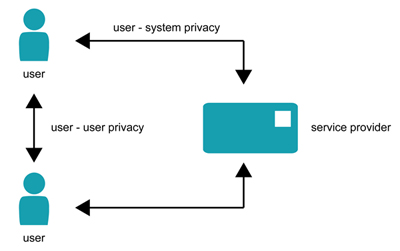
\includegraphics[scale=0.6,keepaspectratio]{fig/user-user-system-privacy}    
  \end{center}     
   \end{figure}
   
In tegenstelling tot sociale netwerken ligt bij aanbevelingssystemen het grootste probleem bij \textit{user-system privacy}. User-system privacy heeft betrekking op privacykwesties tussen de gebruikers en de service provider. Een ander concept in privacy is \emph{deniability of preferences}: de mogelijkheid als gebruiker om eigendom van voorkeuren te ontkennen, of nog dat er geen mogelijkheid kan bestaan om de eigenaar van ratings te identificeren.

\begin{figure}[htpb]   
    \label{Figuur::randomisatie}      
  \begin{center}    
 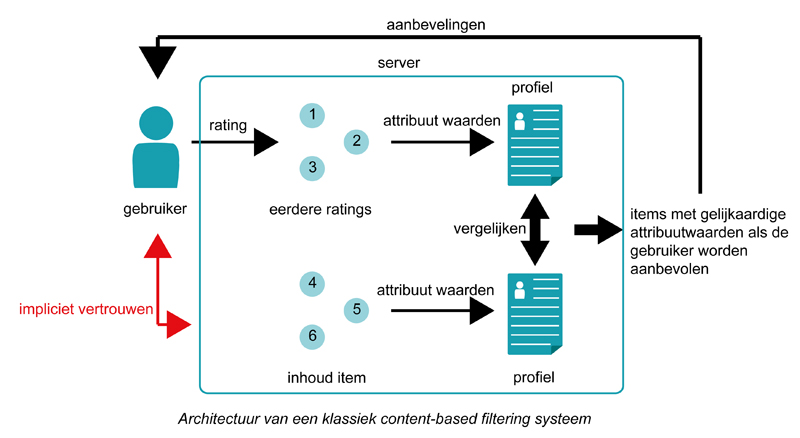
\includegraphics[scale=0.5]{fig/klassiek_systeem}    
  \end{center}   
   
   \end{figure}
Gebruikers hebben vaak een impliciet vertrouwen in de provider om verantwoord met hun data om te springen. 

\section{Betrouwbaarheid}
De betrouwbaarheid van een aanbevelingssysteem leunt dicht aan bij de privacy. Hier kunnen we de volgende vragen stellen : 

\begin{enumerate}
\item Is het systeem voldoende beschermd tegen aanvallen van buitenaf?

 Het aanbevelingssysteem moet allereerst bestand zijn tegen aanvallen van hackers die private informatie willen bemachtigen. In het verleden is er sprake geweest van buitenstaanders die ratings manipuleerden en extra gebruikersprofielen aanmaakten om extra informatie in te winnen over het gedrag van anderen. Een voorbeeld hiervan is een vroege aanval die de correlatieco\"efficient van Pearson misbruikte. De aanval maakte gebruik van het feit dat de co\"efficient $1$ is als twee gebruikers identiek dezelfde ratings hebben. Er werd met behulp van een beetje informatie over de gebruiker een valse account aangemaakt waarmee de co\"efficient $1$ werd. Op deze manier kon men informatie achterhalen over de ratings van de gebruiker.\\
 
 Deze aanvallen kunnnen bemoeilijkt worden door een minder transparant algoritme te gebruiken dat bijvoorbeeld gebruik maakt van Singular Value Decomposition. \\Daarnaast moet het systeem ook voorkomen dat kwaadwillige gebruikers meerdere accounts aanmaken met als doel bepaalde items te promoten of in de vergetelheid te doen belanden. 
 
\item Beveelt het systeem de beste items wel aan?

 Het kan dat een service provider enkel deze items aanbeveelt die in stock zijn of waar de systeemeigenaar het meest geld op verdient, en niet noodzakelijk diegene die het interessantst zijn voor de gebruiker. 
\end{enumerate}

\section{Privacyrisico's bij aanbevelingssystemen}
\label{sec:risicos}

\subsection{De gebruiker onderschat de omvang van de informatie die over hem wordt bijgehouden}
Een gebruiker is zich niet altijd bewust van de omvang van de data die van hem wordt bijgehouden \cite{pirs}. Dit is waarschijnlijk deels zo omdat weinig gebruikers de privacyvoorwaarden lezen vooraleer een applicatie te starten of een account aan te maken bij een bepaalde site. Uit een studie van \citeauthor{privdisc} bij 274 studenten bleek bijvoorbeeld 55.1\% de Facebook privacy policy niet gelezen te hebben \cite{privdisc}. De reden hiervoor was grotendeels omdat de studenten het te veel moeite vonden (43.4\%) of de policy moeilijk te begrijpen vonden (33.6\%). Er is ook gewoonlijk weinig keuze: indien men de voorwaarden niet aanvaardt wordt de toegang tot de applicatie of site ontzegd.
\subsection{Onterecht vertrouwen in de service provider}
\label{onterecht_vertrouwen}

\subsubsection{Het verkopen van data}
Informatie over de ratings en voorkeuren van gebruikers is erg interessant voor marketingdoeleinden. De verkoop van deze gegevens aan derde partijen ligt vaak niet in de lijn der verwachting van de gebruikers. Om de privacy te beschermen wordt deze data vaak geanonimiseerd. Toch biedt deze anonimisatie geen volledige bescherming. Zo hebben \citeauthor{Narayanan2008} in \cite{Narayanan2008} de geanonimiseerde Netflix-database kunnen deanonimiseren: met een heel beperkte kennis van een gebruiker slaagden ze erin om records van die gebruiker uit de databank te halen. Uit deze data konden onder meer politieke voorkeuren en andere gevoelige informatie afgeleid worden.

\subsubsection{Data buiten de verwachte scope \cite{pirs}}
De gebruiker kan ervan uitgaan dat bepaalde informatie enkel zichtbaar is voor een bepaald publiek, terwijl dit niet het geval is. Er is ook geen garantie voor gebruikers dat het personeel van het aanbevelingssysteem geen kijkje neemt in hun persoonlijke data.\\

Informatie op het internet is moeilijk te verwijderen. De service provider vermoeilijkt het soms zelf aangezien er veelal commerci\"ele waarde aan deze gegevens verbonden is. Het kan dus zijn dat data langer aanwezig is dan de gebruiker wil.

\section{Preventie van inbreuken op de privacy}
Nu er inzicht verkregen is welke risico's de gebruiker loopt kan er onderzocht worden wat er kan  gebeuren om inbreuken op zijn privacy te voorkomen.


\subsection{De gebruiker informeren}



